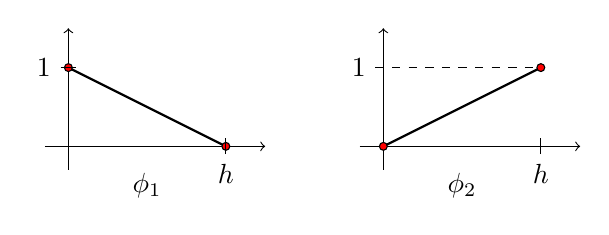
\begin{tikzpicture}
	\def\h{2};

	% PHI 1
	\draw[thick] plot [domain=0:\h] (\x,{1-\x/\h});
	\draw[->] (-.3,0) -- (\h+.5,0);
	\draw[->] (0,-.3) -- (0,1.5);
	\draw[fill=red] (0,1) circle (.05);
	\draw[fill=red] (\h,0) circle (.05);
	\draw (-.1,1) node[left] {$1$} --++(.2,0);
	\draw (\h,-.1) node[below] {$h$} --++(0,.2);
	\draw (\h*.5,-.5) node {$\phi_1$};

	% PHI 2
	\begin{scope}[shift={(\h+2,0)}]
		\draw[thick] plot [domain=0:\h] (\x,{\x/\h});
		\draw[->] (-.3,0) -- (\h+.5,0);
		\draw[->] (0,-.3) -- (0,1.5);
		\draw[fill=red] (0,0) circle (.05);
		\draw[fill=red] (\h,1) circle (.05);
		\draw[dashed] (-.1,1) node[left] {$1$} -- (\h,1);
		\draw (\h,-.1) node[below] {$h$} --++(0,.2);
		\draw (\h*.5,-.5) node {$\phi_2$};
	\end{scope}
\end{tikzpicture}

